\documentclass[tikz,border=10pt]{standalone}
\usepackage{fontspec}
\usepackage[mathrm=sym]{unicode-math}
\setmainfont{texgyrepagella-regular.otf}[
    BoldFont = texgyrepagella-bold.otf,
    ItalicFont = texgyrepagella-italic.otf,
    BoldItalicFont = texgyrepagella-bolditalic.otf
]
\setmathfont{texgyrepagella-math.otf}[AutoFakeBold = 2.5]
\usepackage{tikz}
\usepackage{graphicx}
\usetikzlibrary{arrows.meta, calc}

\graphicspath{{pictures/}{../pictures/}{../../pictures/}}

\begin{document}
\begin{tikzpicture}[>=Stealth, line cap=round, line join=round]

  \def\figW{12.40}
  \def\figH{24.30}

  % Include denoised contour and current base image
  \node[anchor=south west, inner sep=0pt] at (0, 0) {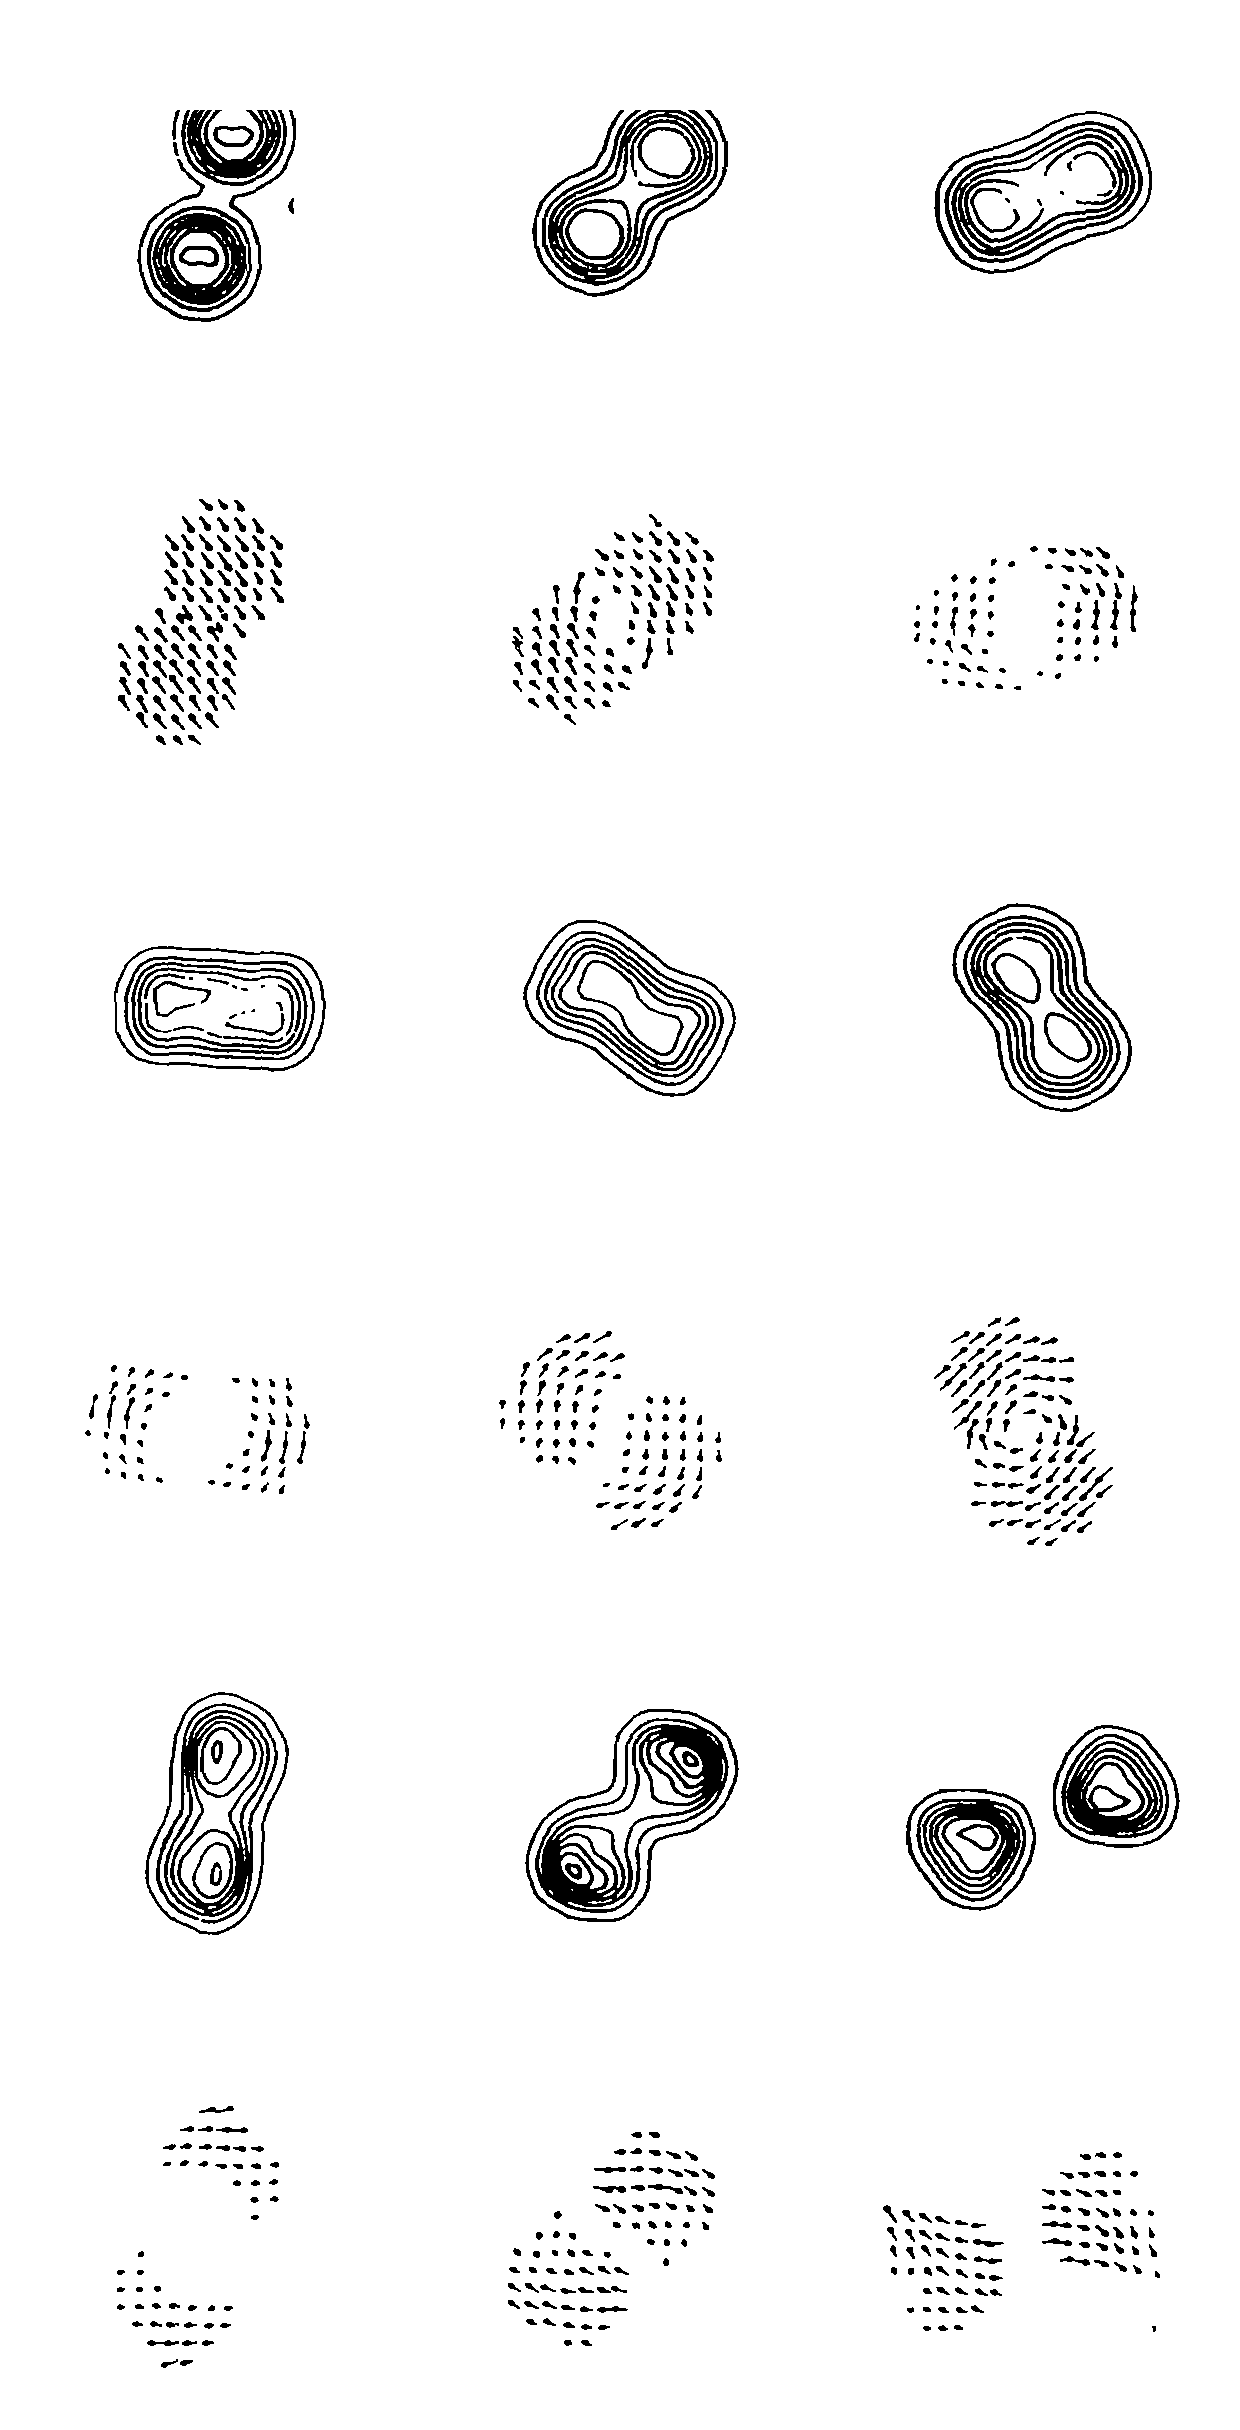
\includegraphics[width=\figW cm, height=\figH cm]{pictures/12_5_base.png}};

  % Outer boundary frame
  \draw[line width=0.85pt] (0, 0) rectangle (\figW, \figH);

  % Vertical internal dividing lines
  \draw[line width=0.55pt] (4.14, 0) -- (4.14, \figH);
  \draw[line width=0.55pt] (8.26, 0) -- (8.26, \figH);

  % Horizontal internal dividing lines
  \draw[line width=0.55pt] (0, 8.10) -- (\figW, 8.10);
  \draw[line width=0.55pt] (0, 16.14) -- (\figW, 16.14);

  % Middle horizontal axis lines in each row
  \draw[line width=0.55pt] (0, 20.22) -- (\figW, 20.22);
  \draw[line width=0.55pt] (0, 12.12) -- (\figW, 12.12);
  \draw[line width=0.55pt] (0, 4.02) -- (\figW, 4.02);

  % Overall title at top (centered over Column 2)
  \node[font=\fontsize{9.5pt}{11.5pt}\selectfont, align=center] at (6.30, \figH + 0.52) {
    ${}^{16}\mathrm{O} + {}^{16}\mathrm{O},\quad E_L/A_P = 8\,\mathrm{MeV}$\\[2pt]
    $b = 5\,\mathrm{fm}$
  };

  % Column centers: Col 1 = 2.16, Col 2 = 6.30, Col 3 = 10.42
  % Row mid axes: Row 1 = 20.22, Row 2 = 12.12, Row 3 = 4.02

  % Time headers above middle axes
  \node[font=\fontsize{8pt}{9pt}\selectfont] at (2.16, 20.52) {$T = 30\,\mathrm{fm}/c$};
  \node[font=\fontsize{8pt}{9pt}\selectfont] at (6.30, 20.52) {$T = 60\,\mathrm{fm}/c$};
  \node[font=\fontsize{8pt}{9pt}\selectfont] at (10.42, 20.52) {$T = 90\,\mathrm{fm}/c$};

  \node[font=\fontsize{8pt}{9pt}\selectfont] at (2.16, 12.42) {$T = 120\,\mathrm{fm}/c$};
  \node[font=\fontsize{8pt}{9pt}\selectfont] at (6.30, 12.42) {$T = 150\,\mathrm{fm}/c$};
  \node[font=\fontsize{8pt}{9pt}\selectfont] at (10.42, 12.42) {$T = 180\,\mathrm{fm}/c$};

  \node[font=\fontsize{8pt}{9pt}\selectfont] at (2.16, 4.32) {$T = 220\,\mathrm{fm}/c$};
  \node[font=\fontsize{8pt}{9pt}\selectfont] at (6.30, 4.32) {$T = 270\,\mathrm{fm}/c$};
  \node[font=\fontsize{8pt}{9pt}\selectfont] at (10.42, 4.32) {$T = 320\,\mathrm{fm}/c$};

  % Middle horizontal ticks and tick numbers (-9, -6, -3, 0, 3, 6, 9)
  \foreach \ymid in {20.22, 12.12, 4.02} {
    \foreach \xc in {2.16, 6.30, 10.42} {
      \foreach \k/\num in {-3/-9, -2/-6, -1/-3, 0/0, 1/3, 2/6, 3/9} {
        \pgfmathsetmacro{\xtick}{\xc + \k * 0.54}
        \draw[line width=0.5pt] (\xtick, \ymid - 0.08) -- (\xtick, \ymid + 0.08);
        \node[below=1.5pt, font=\fontsize{6.5pt}{7.5pt}\selectfont] at (\xtick, \ymid) {$\num$};
      }
      % Calibration velocity vector under tick -9
      \draw[->, line width=0.6pt] ({\xc - 1.62}, {\ymid - 0.44}) -- ({\xc - 1.25}, {\ymid - 0.44});
    }
    % Calibration and Y(fm) labels
    \node[below=0.5pt, font=\fontsize{6.5pt}{7.5pt}\selectfont] at ({2.16 - 1.43}, {\ymid - 0.45}) {$\mathrm{calibration}$};
    \node[below=1pt, font=\fontsize{7.5pt}{8.5pt}\selectfont] at ({2.16 + 1.38}, {\ymid - 0.28}) {$Y(\mathrm{fm})$};
    \node[below=1pt, font=\fontsize{7.5pt}{8.5pt}\selectfont] at ({6.30 + 1.38}, {\ymid - 0.28}) {$Y(\mathrm{fm})$};
  }

  % Z(fm) left vertical axis ticks, numbers, and labels
  % Row 1: Z in [-9, 9] mapped to 20.76 .. 24.00, center Z=0 at 22.38
  % Row 2: Z in [-9, 9] mapped to 12.66 .. 15.90, center Z=0 at 14.28
  % Row 3: Z in [-9, 9] mapped to 4.56 .. 7.80, center Z=0 at 6.18
  \foreach \yc in {22.38, 14.28, 6.18} {
    \foreach \k/\num in {3/9, 2/6, 1/3, 0/0, -1/-3, -2/-6, -3/-9} {
      \pgfmathsetmacro{\ytick}{\yc + \k * 0.54}
      \draw[line width=0.5pt] (0, \ytick) -- (-0.09, \ytick);
      \node[left=1.5pt, font=\fontsize{7pt}{8pt}\selectfont] at (-0.09, \ytick) {$\num$};
    }

    % Z(fm) label centered vertically at Z=0
    \node[left=18pt, font=\fontsize{9pt}{10pt}\selectfont] at (0, \yc) {$Z(\mathrm{fm})$};

    % Inward tick marks at Z=0 on dividers and right border
    \draw[line width=0.5pt] (4.14 - 0.08, \yc) -- (4.14 + 0.08, \yc);
    \draw[line width=0.5pt] (8.26 - 0.08, \yc) -- (8.26 + 0.08, \yc);
    \draw[line width=0.5pt] (\figW, \yc) -- (\figW - 0.08, \yc);
  }

  % In-panel text labels
  % Row 1
  \node[font=\fontsize{8pt}{9pt}\selectfont] at (3.26, 22.38) {$\mathit{density}$};
  \node[font=\fontsize{8pt}{9pt}\selectfont] at (3.26, 18.25) {$\mathit{current}$};

  % Row 2
  \node[font=\fontsize{8pt}{9pt}\selectfont] at (2.16, 15.15) {$\mathit{density}$};
  \node[font=\fontsize{8pt}{9pt}\selectfont] at (2.16, 10.95) {$\mathit{current}$};

  % Row 3
  \node[font=\fontsize{8pt}{9pt}\selectfont] at (3.26, 6.18) {$\mathit{density}$};
  \node[font=\fontsize{8pt}{9pt}\selectfont] at (3.26, 2.05) {$\mathit{current}$};

\end{tikzpicture}
\end{document}
